\section{Spectrum of Autoregressive Processes}
\subsection{Shortcomings of unbiased ACF}
Based on the Yule-Walker equations, the autoregressive parameters can be obtained by the inversion of autocorrelation matrix, as expressed in Eq.\ref{proof:ar}.
\begin{equation}
\mathbf{r}_{xx}=\mathbf R_{xx}\mathbf a \quad \Rightarrow \quad \mathbf a=\mathbf R^{-1}_{xx}\mathbf {r}_{xx}
\label{proof:ar}
\end{equation}
Therefore, the ACF matrix $\mathbf {R}_{xx}$ is positive semi-definite for biased estimator which is invertible. As to unbiased ACF shown in previous section, the autocorrelation matrix may be singular which can not be inverted.
\subsection{AR Modelling with few samples}
Given the autoregressive parameters $\mathbf a$ =[2.76 -3.81 2.65 -0.92] and the white noise power $\sigma^2=1$, the estimation of AR modelling process with the order $p$ from 2 to 14 is shown in Fig.\ref{fig:1_4_b}. The AR model has a frustrated performance with low order which only detects one peak. With the order increasing, the estimation is approaching to the actual frequency response. However, the AR(4) model perform poorly although it consists with the true order of filter. This is probably caused by the small number of available samples with $N=500$. Therefore, in order to obtain desirable response, either the order of AR model or the number of sample should increase. 
\begin{figure}[htbp]
     \centering
     \begin{subfigure}[b]{0.35\textwidth}
         \centering
         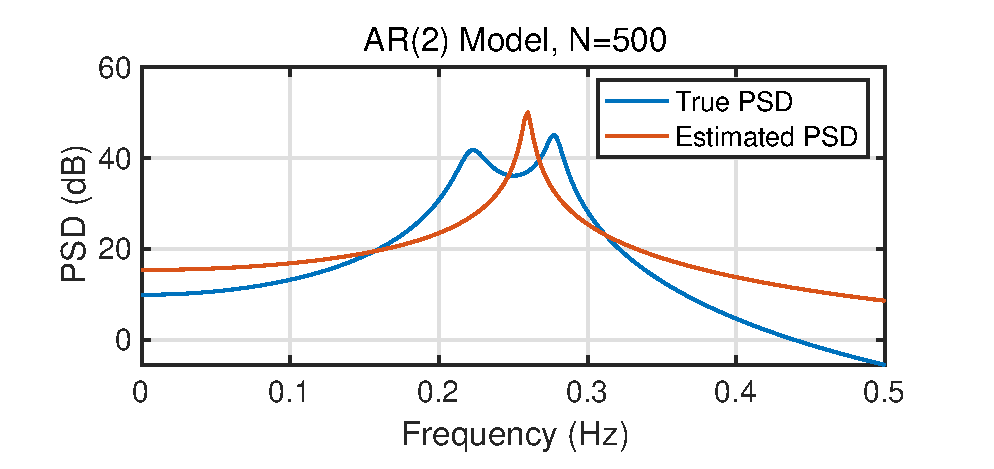
\includegraphics[width=\textwidth]{fig/14/14b1.eps}
     \end{subfigure}
     ~
     \begin{subfigure}[b]{0.35\textwidth}
         \centering
         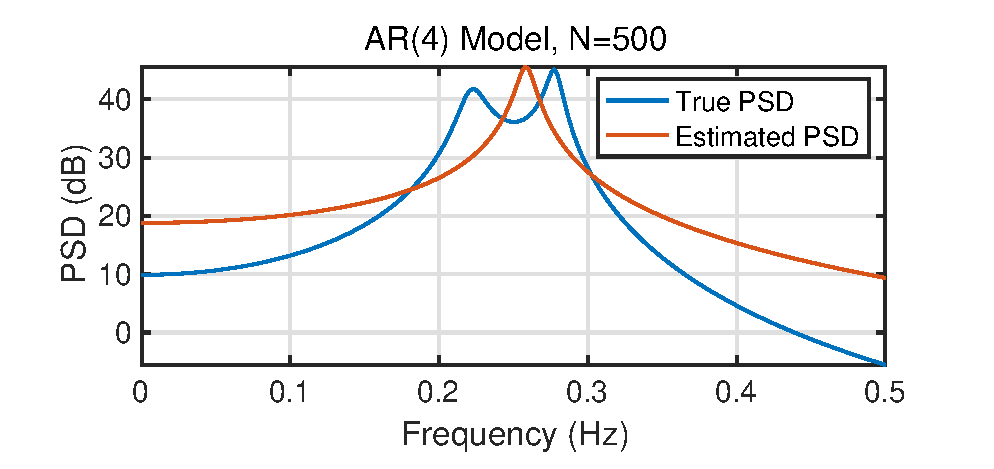
\includegraphics[width=\textwidth]{fig/14/14b2.eps}
     \end{subfigure}
     ~
     \begin{subfigure}[b]{0.35\textwidth}
         \centering
         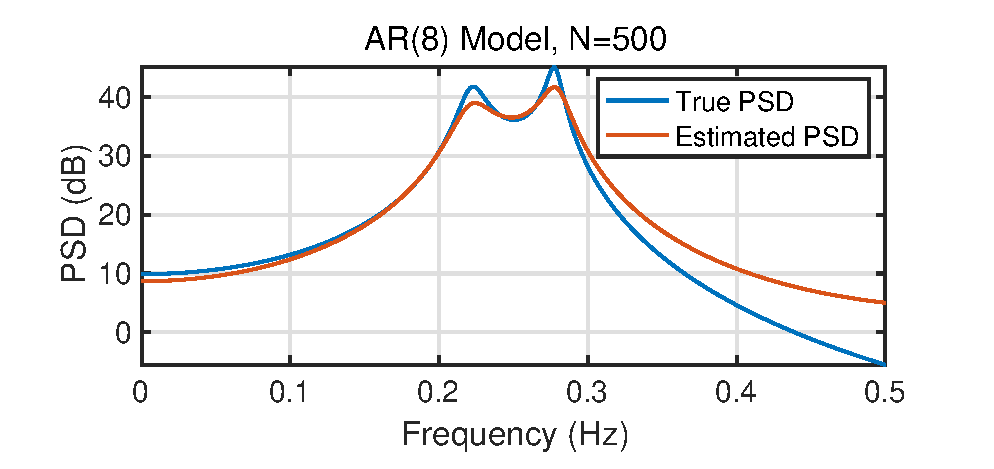
\includegraphics[width=\textwidth]{fig/14/14b3.eps}
     \end{subfigure}
     ~
     \begin{subfigure}[b]{0.35\textwidth}
         \centering
         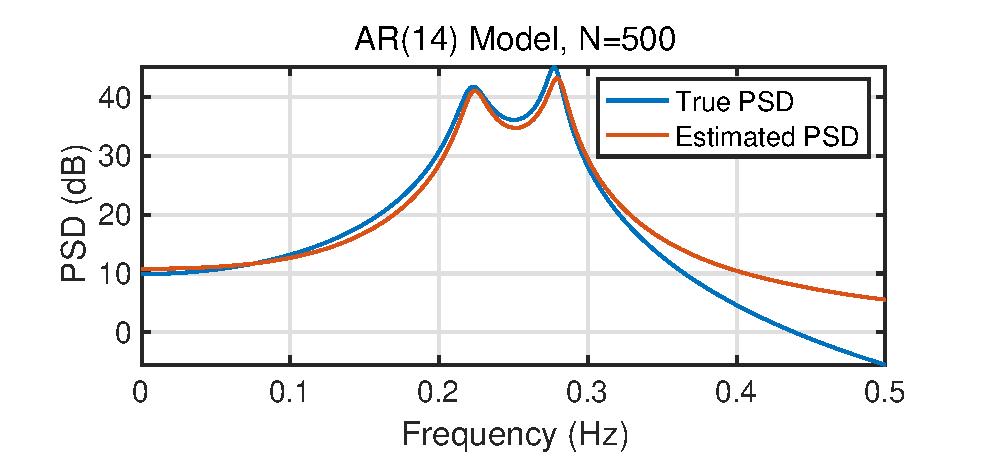
\includegraphics[width=\textwidth]{fig/14/14b4.eps}
     \end{subfigure}
        \caption{AR Model with varying order}
        \label{fig:1_4_b}
\end{figure}
\subsection{AR modelling with increasing samples}
Repeat the process in previous section except applying $10k$ samples to model. When the AR order $p < p_{actrual =4}$, the autoregressive parameters can not be estimated. As shown in Fig.\ref{fig:1_4_c}, the AR(2) model only captures one peak frequency, which is an under-modelling estimation. However, the AR model matches the actual response with two peaks when the order $p$ is larger than 4. Moreover, increasing order ($p>5$) brought less improvement between actual response and estimation. Therefore, the optimal order for the large number of sample is $4^{th}$.
\begin{figure}[htbp]
     \centering
     \begin{subfigure}[b]{0.35\textwidth}
         \centering
         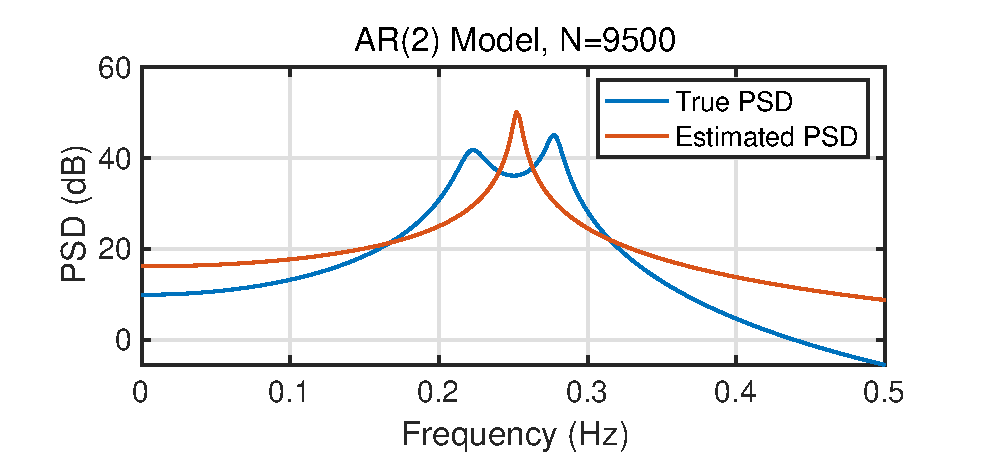
\includegraphics[width=\textwidth]{fig/14/14c1.eps}
     \end{subfigure}
     ~
     \begin{subfigure}[b]{0.35\textwidth}
         \centering
         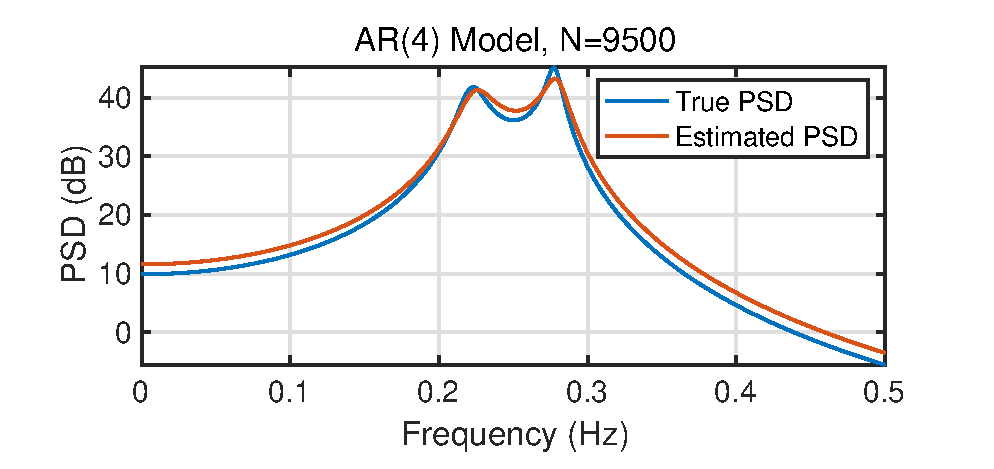
\includegraphics[width=\textwidth]{fig/14/14c2.eps}
     \end{subfigure}
     ~
     \begin{subfigure}[b]{0.35\textwidth}
         \centering
         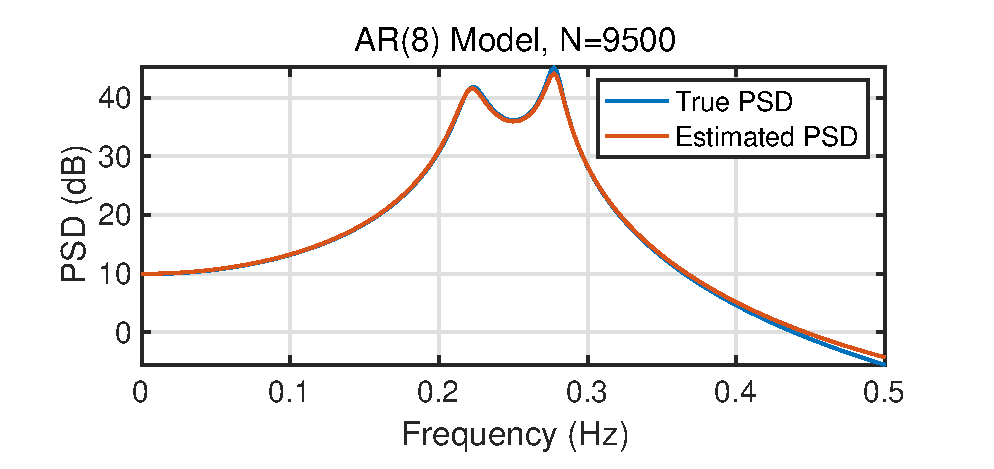
\includegraphics[width=\textwidth]{fig/14/14c3.eps}
     \end{subfigure}
     ~
     \begin{subfigure}[b]{0.35\textwidth}
         \centering
         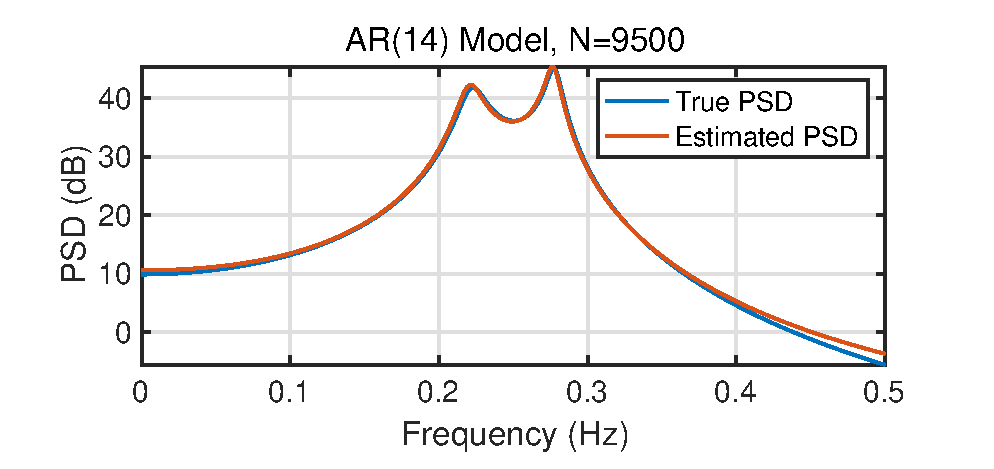
\includegraphics[width=\textwidth]{fig/14/14c4.eps}
     \end{subfigure}
        \caption{AR Modelling with $10k$ samples}
        \label{fig:1_4_c}
\end{figure}
